\FloatBarrier
\Needspace{16\baselineskip}
\section{Релевантность и вознаграждение}

В таблице приведены средние метрик трёх отдельных запусков,
предсказанные вероятности моделей не усредняются.
NDCG@10 и Recall@10 сравнивают выдачу с наблюдавшимися действиями,
основная RM и аудитор предсказывают дослушивание предлагаемых объектов.
Ожидаемая награда первого шага оценена по 32 действиям на запрос
с общими случайными числами для всех политик

\begin{table}[!htbp]
\centering
\small
\setlength{\tabcolsep}{4pt}
\setlength{\reporttablewidth}{\dimexpr\linewidth-32pt\relax}
\begin{tabular}{@{}>{\raggedright\arraybackslash}p{0.36000\reporttablewidth}>{\raggedright\arraybackslash}p{0.16000\reporttablewidth}>{\raggedright\arraybackslash}p{0.16000\reporttablewidth}>{\raggedright\arraybackslash}p{0.16000\reporttablewidth}>{\raggedright\arraybackslash}p{0.16000\reporttablewidth}@{}}
\toprule
Модель & NDCG@10 & Recall@10 & Основная RM & Аудитор \\
\midrule
Популярность & 0.00169 & 0.00309 & 0.6471 & 0.6487 \\
Частота в контексте & 0.00490 & 0.00842 & 0.6944 & 0.6816 \\
SFT GPT-2 & 0.00688 & 0.01542 & 0.6925 & 0.6780 \\
Continued-CE & 0.00686 & 0.01546 & 0.6923 & 0.6778 \\
Completion, $\beta=0$ & 0.00157 & 0.00326 & 0.7346 & 0.6940 \\
Completion, $\beta=0.05$ & 0.00669 & 0.01316 & 0.7089 & 0.6867 \\
Completion, $\beta=0.20$ & 0.00706 & 0.01494 & 0.6981 & 0.6809 \\
Seconds, $\beta=0.10$ & 0.00553 & 0.01167 & 0.6906 & 0.6763 \\
Balanced, $\beta=0.10$ & 0.00679 & 0.01505 & 0.6953 & 0.6794 \\
Bandit, $\beta=0.05$ & 0.00725 & 0.01544 & 0.7058 & 0.6851 \\
\bottomrule
\end{tabular}
\caption{Test на общих запросах и полном словаре, два последних столбца показывают прогноз дослушивания}
\label{tab:rl-main}
\end{table}

В основном сравнении balanced с continued-CE разность NDCG@10
равна \(-0.00008\) с парным 95\% интервалом
\([-0.00107,+0.00084]\). Прогноз дослушивания вырос на
0.00297 \([+0.00264,+0.00328]\) по основной RM
и на 0.00158 \([+0.00136,+0.00180]\) по аудитору

Здесь и далее приведены парные 95\% интервалы.
В основном сравнении бутстрэп выполнен по 434 пользователям с 2\,000 перевыборками,
сначала метрики каждого запроса усреднены по одинаковым seed.
Все запросы выбранного пользователя переносятся вместе.
Интервалы условны на трёх обучениях и использованных случайных числах.
Они подтверждают рост модельной награды, но не рост релевантности

Потеря 5\% NDCG@10 continued-CE соответствует 0.00034,
интервал разности заметно шире. Поэтому близость точечных оценок
не доказывает сохранение качества в этом допуске.
Порог 95\% при выборе модели не заменяет проверку допустимой потери на test

\begin{figure}[!htbp]
\centering
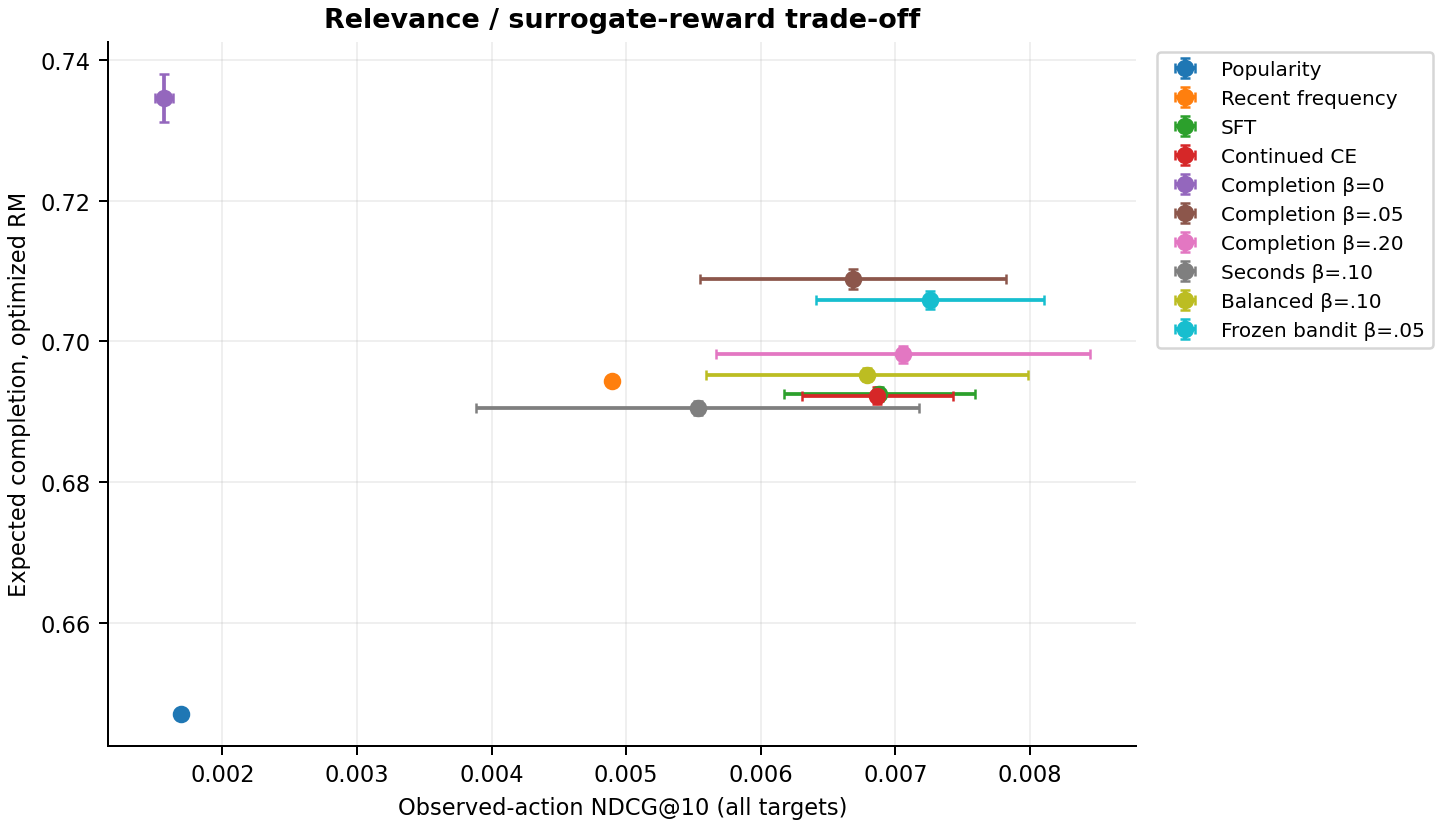
\includegraphics[width=\linewidth,height=.32\textheight,keepaspectratio]{figures/pareto.png}
\caption{Компромисс между NDCG@10 и прогнозом дослушивания, отрезки показывают стандартное отклонение трёх запусков}
\label{fig:rl-pareto}
\end{figure}
